\documentclass{article}
\usepackage{tikz}
\usetikzlibrary{positioning}
\usetikzlibrary{shapes.geometric}
\usetikzlibrary{shapes.symbols}
\usetikzlibrary{shadows}
\usetikzlibrary{arrows}

\pagestyle{empty}

\newcommand{\ctpstyle}[0]{
  \tikzstyle{node}=[circle,draw] 
  \tikzstyle{source}=[node,thick]
  \tikzstyle{target}=[node,thick]
  \tikzstyle{edge}=[->] 
  \tikzstyle{elbl}=[sloped,midway,above]}

\newcommand{\ctpmin}[1]{
	\node[source] (s) at (0,0) {s};
	\node[target] (t) at (5,0) {t};
	\node[node] (v) at (2.5,1.5) {v};
	\draw[edge,bend right] (s) to node[elbl] {$3$} (t);
	\draw[edge,bend left] (s) to node[elbl] {$0.5$} (v);
	#1 }


\begin{document}

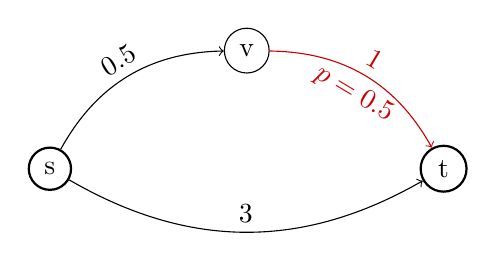
\begin{tikzpicture}
\ctpstyle
\ctpmin{
  	\draw[edge,bend left,red!80!black] (v) to node[elbl] {$1$} node[elbl,below] {$p=0.5$} (t); }
\end{tikzpicture}

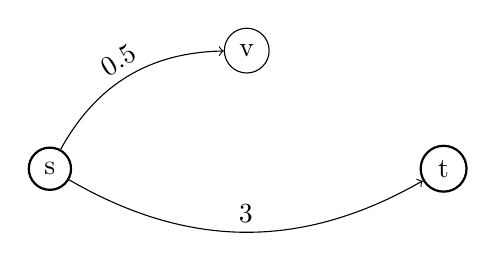
\begin{tikzpicture}
\ctpstyle
\ctpmin{}
\end{tikzpicture}

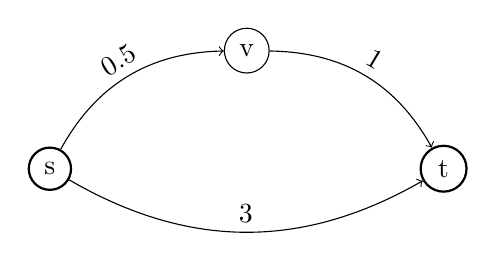
\begin{tikzpicture}
\ctpstyle
\ctpmin{
  	\draw[edge,bend left] (v) to node[elbl] {$1$} (t); }
\end{tikzpicture}

\end{document}
